
\documentclass[14pt]{article}
\usepackage{amsmath}
\usepackage{latexsym}
\usepackage{amsfonts}
\usepackage[normalem]{ulem}
\usepackage{soul}
\usepackage{array}
\usepackage{amssymb}
\usepackage{extarrows}
\usepackage{graphicx}
\usepackage[backend=biber,
style=numeric,
sorting=none,
isbn=false,
doi=false,
url=false,
]{biblatex}\addbibresource{bibliography-biblatex.bib}

\usepackage{subfig}
\usepackage{wrapfig}
\usepackage{wasysym}
\usepackage{enumitem}
\usepackage{adjustbox}
\usepackage{ragged2e}
\usepackage[svgnames,table]{xcolor}
\usepackage{tikz}
\usepackage{longtable}
\usepackage{changepage}
\usepackage{setspace}
\usepackage{hhline}
\usepackage{multicol}
\usepackage{tabto}
\usepackage{float}
\usepackage{multirow}
\usepackage{makecell}
\usepackage{fancyhdr}
\usepackage[toc,page]{appendix}
\usepackage[hidelinks]{hyperref}
\usetikzlibrary{shapes.symbols,shapes.geometric,shadows,arrows.meta}
\tikzset{>={Latex[width=1.5mm,length=2mm]}}
\usepackage{flowchart}\usepackage[paperheight=11.0in,paperwidth=8.5in,left=1.0in,right=0.88in,top=1.5in,bottom=1.5in,headheight=1in]{geometry}
\usepackage[utf8]{inputenc}
\usepackage[T1]{fontenc}
\TabPositions{0.5in,1.0in,1.5in,2.0in,2.5in,3.0in,3.5in,4.0in,4.5in,5.0in,5.5in,6.0in,6.5in,}

\urlstyle{same}

\renewcommand{\_}{\kern-1.5pt\textunderscore\kern-1.5pt}



\setcounter{tocdepth}{5}
\setcounter{secnumdepth}{5}


\setlistdepth{9}
\renewlist{enumerate}{enumerate}{9}
		\setlist[enumerate,1]{label=\arabic*)}
		\setlist[enumerate,2]{label=\alph*)}
		\setlist[enumerate,3]{label=(\roman*)}
		\setlist[enumerate,4]{label=(\arabic*)}
		\setlist[enumerate,5]{label=(\Alph*)}
		\setlist[enumerate,6]{label=(\Roman*)}
		\setlist[enumerate,7]{label=\arabic*}
		\setlist[enumerate,8]{label=\alph*}
		\setlist[enumerate,9]{label=\roman*}

\renewlist{itemize}{itemize}{9}
		\setlist[itemize]{label=$\cdot$}
		\setlist[itemize,1]{label=\textbullet}
		\setlist[itemize,2]{label=$\circ$}
		\setlist[itemize,3]{label=$\ast$}
		\setlist[itemize,4]{label=$\dagger$}
		\setlist[itemize,5]{label=$\triangleright$}
		\setlist[itemize,6]{label=$\bigstar$}
		\setlist[itemize,7]{label=$\blacklozenge$}
		\setlist[itemize,8]{label=$\prime$}

\setlength{\topsep}{0pt}\setlength{\parindent}{0pt}


\renewcommand{\arraystretch}{1.3}

\begin{document}
\begin{Center}
{\fontsize{22pt}{27.2pt}\selectfont Design and Analysis of Algorithms Assignment-3}
\end{Center}

\vspace{\baselineskip}
\begin{Center}
{\fontsize{17pt}{20.4pt}\selectfont Indian Institute of Information Technology, Allahabad}
\end{Center}
\begin{Center}
{\fontsize{17pt}{20.4pt}\selectfont Department of Information Technology}
\end{Center}

\vspace{\baselineskip}

\vspace{\baselineskip}

\vspace{\baselineskip}


%%%%%%%%%%%%%%%%%%%% Table No: 1 starts here %%%%%%%%%%%%%%%%%%%%


\begin{table}[H]
 			\centering
\begin{tabular}{p{1.97in}p{1.97in}p{1.97in}}
\hline
%row no:1
\multicolumn{1}{|p{1.97in}}{\Centering {\fontsize{13pt}{15.6pt}\selectfont \textbf{Somesh Kumar Maurya}} \par \Centering {\fontsize{13pt}{15.6pt}\selectfont \textbf{IIT2019081}} \par \Centering {\fontsize{13pt}{15.6pt}\selectfont \textbf{IIT2019081@iiita.ac.in}}} & 
\multicolumn{1}{|p{1.97in}}{\Centering {\fontsize{13pt}{15.6pt}\selectfont \textbf{Navdeep Kumar}} \par \Centering {\fontsize{13pt}{15.6pt}\selectfont \textbf{IIT2019082}} \par \Centering {\fontsize{13pt}{15.6pt}\selectfont \textbf{IIT2019082@iiita.ac.in}}} & 
\multicolumn{1}{|p{1.97in}|}{\Centering {\fontsize{13pt}{15.6pt}\selectfont \textbf{Sumit Bakoliya}} \par \Centering {\fontsize{13pt}{15.6pt}\selectfont \textbf{IIT2019083}} \par \Centering {\fontsize{13pt}{15.6pt}\selectfont \textbf{IIT2019083@iiita.ac.in}}} \\
\hhline{---}

\end{tabular}
 \end{table}


%%%%%%%%%%%%%%%%%%%% Table No: 1 ends here %%%%%%%%%%%%%%%%%%%%


\vspace{\baselineskip}
\begin{multicols}{2}
\begin{justify}
\textbf{\ \ \  Abstract: Given an n x n matrix, where every row and column is sorted in increasing order. Given a key, how to decide whether this key is in the matrix. \\
In this paper, the problem has been solved by using a divide and conquer approach by dividing a given big problem into 4 smaller subproblems and implementing it recursively using concept of recursion.}
\end{justify}

\vspace{\baselineskip}

\vspace{\baselineskip}
\begin{enumerate}
	\item {\fontsize{15pt}{18.0pt}\selectfont \textbf{INTRODUCTION}}

\vspace{\baselineskip}
\begin{justify}
Divide and Conquer is an algorithm design paradigm in which we recursively break down a problem into two or more sub-problems of the same or related type, until these subproblems become simple enough to be solved directly.
\end{justify}
\begin{justify}
The solutions to the sub-problems are then combined to give a solution to the original problem.
\end{justify}
\begin{justify}
The divide-and-conquer paradigm is often used to find an optimal solution of a problem in which we recursively simplify the problem by decreasing the constraints of a subproblem and selecting / dis-selecting a given subproblem based on some conditions.
\end{justify}

\vspace{\baselineskip}

\vspace{\baselineskip}

\vspace{\baselineskip}
	\item {\fontsize{15pt}{18.0pt}\selectfont \textbf{ALGORITHM DESIGN}}

\vspace{\baselineskip}
\begin{justify}
{\fontsize{12pt}{14.4pt}\selectfont \textbf{OVERVIEW:}}
\end{justify}
\begin{justify}
At first, the size of the matrix is inserted and then using a random function a matrix is generated. Now the number of keys to be checked is inserted and then that number of keys is inserted.
\end{justify}
\begin{justify}
Now for finding whether the key is present in the matrix or not, we have used the following procedure.
\end{justify}

\vspace{\baselineskip}
\begin{justify}
\textbf{\uline{Step 1: Generating function call}} A function named check is created which contains parameters left x coordinate (lx), left y coordinate (ly), right x coordinate (rx), right y coordinate (ry) and key to be checked.
\end{justify}
\begin{justify}
A particular value of lx,ly,rx,ry,key means to check for the key to be present in column lx+1 to rx and in row ly+1 to ry.
\end{justify}

\vspace{\baselineskip}
\begin{justify}
\textbf{\uline{Step 2: Checking Base condition}}\  The several base condition to be checked are:
\end{justify}
\begin{enumerate}
	\item If the given row column pair does not contain any value i.e. number of elements is 0, then return false.
	\item  If the given row column pair contains a single value i.e. number of elements is 1, then return true if the element is equal to key else return false.
	\item If the biggest element in the row column pair is less than the key element or the smallest element in the row column pair is greater than the key element, then return false else check for subproblems.
\end{enumerate}

\vspace{\baselineskip}
\begin{justify}
\textbf{\uline{Step 3: Function call for subproblems}}\  If the given problem has row range from ly to ry and column range from lx to rx, then consider mid x coordinate mx=(lx+rx)/2 and mid y coordinate my=(ly+ry)/2.
\end{justify}
\begin{justify}
Now function call for all 4 subproblems by using this pair of midpoint i.e. (lx,ly,mx,my) , (mx,ly,rx,my) , (lx,my,mx,ry) , (mx,my,rx,ry) .
\end{justify}

\vspace{\baselineskip}

\vspace{\baselineskip}
\begin{justify}
{\fontsize{12pt}{14.4pt}\selectfont \textbf{ALGORITHM DESCRIPTION :}}
\end{justify}

\vspace{\baselineskip}
\begin{justify}
Let the numbers be stored in a matrix mat and size of the matrix is stored in n and assuming all rows and columns are sorted in increasing order.
\end{justify}
\begin{justify}
function prototype is
\end{justify}
\begin{justify}
bool check( int lx , int ly , int rx , int ry , int key)
\end{justify}

\vspace{\baselineskip}
\begin{justify}
\textbf{\uline{Step 1: Generating function call}} 
\end{justify}

\vspace{\baselineskip}
\begin{justify}
int key
\end{justify}
\begin{justify}
cin>>key
\end{justify}
\begin{justify}
bool ans = check(0,0,n,n,key)
\end{justify}
\begin{justify}
if(ans\ is\ true)   Key is present
\end{justify}
\begin{justify}
else\ \ \  Key is not present
\end{justify}

\vspace{\baselineskip}

\vspace{\baselineskip}
\begin{justify}
\textbf{\uline{Step 2: Checking Base condition}} 
\end{justify}

\vspace{\baselineskip}
\begin{justify}
if(lx==rx $ \vert $ $ \vert $  ly==ry)return false
\end{justify}
\begin{justify}
if(rx-lx==1 $\&$ $\&$  ry-ly==1)
\end{justify}
\begin{justify}
\ \ \ \ \ \ \  if(mat[rx][ry]==key)return true
\end{justify}
\begin{justify}
\ \ \ \ \ \ \  else return false
\end{justify}
\begin{justify}
if(mat[lx][ly]>key $ \vert $ $ \vert $  mat[rx][ry]<key )return false
\end{justify}

\vspace{\baselineskip}
\begin{justify}
\textbf{\uline{Step 3: Function call for subproblems}} 
\end{justify}
\begin{justify}
mx=(lx+rx)/2
\end{justify}
\begin{justify}
my=(ly+ry)/2
\end{justify}
\begin{justify}
bool ans=false
\end{justify}
\begin{justify}
ans$ \vert $ =check(lx,ly,mx,my,key)
\end{justify}
\begin{justify}
ans$ \vert $ =check(mx,ly,rx,my,key)
\end{justify}
\begin{justify}
ans$ \vert $ =check(lx,my,mx,ry,key)
\end{justify}
\begin{justify}
ans$ \vert $ =check(mx,my,rx,ry,key)
\end{justify}
\begin{justify}
return ans
\end{justify}

\vspace{\baselineskip}

\vspace{\baselineskip}
\begin{justify}
\textbf{For example: }Assuming the matrix to be
\end{justify}
\begin{justify}
\ 0\ \ 1\ \ 2\ \ 3\ \ 4  5  6  7  8  9
\end{justify}
\begin{justify}
10 11 12 13 14 15 16 17 18 19 
\end{justify}
\begin{justify}
20 21 22 23 24 25 26 27 28 29 
\end{justify}
\begin{justify}
30 31 32 33 34 35 36 37 38 39 
\end{justify}
\begin{justify}
40 41 42 43 44 45 46 47 48 49 
\end{justify}
\begin{justify}
50 51 52 53 54 55 56 57 58 59 
\end{justify}
\begin{justify}
60 61 62 63 64 65 66 67 68 69 
\end{justify}
\begin{justify}
70 71 72 73 74 75 76 77 78 79 
\end{justify}
\begin{justify}
80 81 82 83 84 85 86 87 88 89 
\end{justify}
\begin{justify}
90 91 92 93 94 95 96 97 98 99 
\end{justify}
\begin{justify}
n=10
\end{justify}
\begin{justify}
Searching for key 81
\end{justify}

\vspace{\baselineskip}
\begin{justify}
check( 0 , 0 , 10 , 10 , 81)
\end{justify}
\begin{justify}
mx=5\  my=5
\end{justify}
\begin{justify}
check( 0 , 0 , 5 , 5 , 81) 
\end{justify}
\begin{justify}
Does not contain key so return false
\end{justify}
\begin{justify}
check( 5 , 0 , 10 , 5 , 81) 
\end{justify}
\begin{justify}
Does not contain key so return false
\end{justify}
\begin{justify}
check( 0 , 5 , 5 , 10 , 81) 
\end{justify}
\begin{justify}
Contain key, checking further
\end{justify}
\begin{justify}
check( 5 , 5 , 10 , 10 , 81)
\end{justify}
\begin{justify}
Does not contain key so return false
\end{justify}

\vspace{\baselineskip}
\begin{justify}
check( 0 , 5 , 5 , 10 , 81) 
\end{justify}
\begin{justify}
mx=2\  my=7
\end{justify}
\begin{justify}
check( 0 , 5 , 2 , 7 , 81) 
\end{justify}
\begin{justify}
Does not contain key so return false
\end{justify}
\begin{justify}
check( 2 , 5 , 5 , 7 , 81) 
\end{justify}
\begin{justify}
Does not contain key so return false
\end{justify}
\begin{justify}
check( 0 , 7 , 2 , 10 , 81) 
\end{justify}
\begin{justify}
Contain key, checking further
\end{justify}
\begin{justify}
check( 2 , 7 , 5 , 10 , 81) 
\end{justify}
\begin{justify}
Does not contain key so return false
\end{justify}

\vspace{\baselineskip}
\begin{justify}
check( 0 , 7 , 2 , 10 , 81) 
\end{justify}
\begin{justify}
mx=1\  my=8
\end{justify}
\begin{justify}
check( 0 , 7 , 1 , 8 , 81) 
\end{justify}
\begin{justify}
Does not contain key so return false
\end{justify}
\begin{justify}
check( 1 , 7 , 2 , 8 , 81) 
\end{justify}
\begin{justify}
Does not contain key so return false
\end{justify}
\begin{justify}
check( 0 , 8 , 1 , 10 , 81) 
\end{justify}
\begin{justify}
Does not contain key so return false
\end{justify}
\begin{justify}
check( 1 , 8 , 2 , 10 , 81)
\end{justify}
\begin{justify}
Contain key, checking further
\end{justify}

\vspace{\baselineskip}
\begin{justify}
check( 1 , 8 , 2 , 10 , 81)
\end{justify}
\begin{justify}
mx=1\  my=9
\end{justify}
\begin{justify}
check( 1 , 8 , 1 , 9 , 81) 
\end{justify}
\begin{justify}
lx==rx\ \  so return false
\end{justify}
\begin{justify}
check( 1 , 8 , 2 , 9 , 81) 
\end{justify}
\begin{justify}
\textbf{mat[2][9]==key\ \ \  so return true}
\end{justify}
\begin{justify}
check( 1 , 9 , 1 , 10 , 81) 
\end{justify}
\begin{justify}
lx==rx\ \  so return false
\end{justify}
\begin{justify}
check( 1 , 9 , 2 , 10 , 81)
\end{justify}
\begin{justify}
mat[2][10]!=key\ \ \  so return false
\end{justify}

\vspace{\baselineskip}

\vspace{\baselineskip}

\vspace{\baselineskip}

\vspace{\baselineskip}
	\item {\fontsize{15pt}{18.0pt}\selectfont \textbf{ALGORITHM ANALYSIS}}

\vspace{\baselineskip}
\begin{justify}
For the analysis of algorithm we break the code snippet into several segments and count the number of addition, subtraction, multiplication, division, assign, comparison and by considering all those operations as 1 unit of operation, we will try to find the overall time complexity of the algorithm by multiplying total number of operations into number of times the code segment is running in the algorithm.
\end{justify}
\begin{justify}
For the space complexity we tend to count the total amount of space taken by that algorithm to implement and then find a relation between the amount of space required and the input. The time and space complexity analysis for various steps is as shown below.
\end{justify}

\vspace{\baselineskip}
\vspace{\baselineskip}
\begin{justify}
\textbf{\uline{Step 1: Generating function call}} 
\end{justify}

\vspace{\baselineskip}
\begin{justify}
int key
\end{justify}
\begin{justify}
cin>>key
\end{justify}
\begin{justify}
bool ans = check(0,0,n,n,key)
\end{justify}
\begin{justify}
if(ans\ is\ true)   Key is present
\end{justify}
\begin{justify}
else\ \ \  Key is not present
\end{justify}

\vspace{\baselineskip}
\begin{itemize}
	\item Number of operation = 7
	\item Frequency = number of function call

\vspace{\baselineskip}

\vspace{\baselineskip}
\begin{justify}
\textbf{\uline{Step 2: Checking Base condition}} 
\end{justify}

\vspace{\baselineskip}
\begin{justify}
if(lx==rx $ \vert $ $ \vert $  ly==ry)return false
\end{justify}
\begin{justify}
if(rx-lx==1 $\&$ $\&$  ry-ly==1)
\end{justify}
\begin{justify}
\ \ \ \ \ \ \  if(mat[rx][ry]==key)return true
\end{justify}
\begin{justify}
\ \ \ \ \ \ \  else return false
\end{justify}
\begin{justify}
if(mat[lx][ly]>key $ \vert $ $ \vert $  mat[rx][ry]<key )return false
\end{justify}

\vspace{\baselineskip}
	\item Number of operation = 4+5+3+6
	\item Frequency = number of function call

\vspace{\baselineskip}
\begin{justify}
\textbf{\uline{Step 3: Function call for subproblems}} 
\end{justify}

\vspace{\baselineskip}
\begin{justify}
mx=(lx+rx)/2
\end{justify}
\begin{justify}
my=(ly+ry)/2
\end{justify}
\begin{justify}
bool ans=false
\end{justify}
\begin{justify}
ans$ \vert $ =check(lx,ly,mx,my,key)
\end{justify}
\begin{justify}
ans$ \vert $ =check(mx,ly,rx,my,key)
\end{justify}
\begin{justify}
ans$ \vert $ =check(lx,my,mx,ry,key)
\end{justify}
\begin{justify}
ans$ \vert $ =check(mx,my,rx,ry,key)
\end{justify}
\begin{justify}
return ans
\end{justify}

\vspace{\baselineskip}
	\item Number of operation = 3+3+1+4+1
	\item Frequency = number of function call
\end{itemize}
\begin{justify}
\textbf{Number of function calls}
\end{justify}
\begin{justify}
In\ the\ worst case all elements in the matrix are equal. In that case the number of function calls will be ( n$\ast$ n/1 ) + ( n$\ast$ n/4 ) + ( n$\ast$ n/16 ) + $ \ldots $ . + 1  =  n$\ast$ n$\ast$ 4/3
\end{justify}
\begin{justify}
Thus the total number of function calls are proportional to n$ \string^ $ 2
\end{justify}


\begin{justify}
Total number of operations for this algorithm\textbf{ }
\end{justify}
\begin{justify}
= 37 $\ast$  ( n$\ast$ n$\ast$ 4/3 )
\end{justify}
\begin{justify}
{\fontsize{12pt}{14.4pt}\selectfont $\propto$  } n$ \string^ $ 2
\end{justify}
\begin{justify}
Thus \textbf{time complexity = O (n$ \string^ $ 2)}
\end{justify}

\vspace{\baselineskip}
\begin{justify}
Total Number of variables used is
\end{justify}
\begin{justify}
= (2+1) $\ast$  number of function call
\end{justify}
\begin{justify}
= 3 $\ast$  ( n$\ast$ n$\ast$ 4/3 )
\end{justify}
\begin{justify}
{\fontsize{12pt}{14.4pt}\selectfont $\propto$  } n$ \string^ $ 2
\end{justify}
\begin{justify}
Thus \textbf{space\ complexity is  O (n$ \string^ $ 2)}
\end{justify}

\vspace{\baselineskip}
\begin{justify}
The best case is for n=1
\end{justify}
\begin{justify}
For\  n=1 number of operation = constant
\end{justify}
\begin{justify}
Thus \textbf{time\textsubscript{min}= \(  \Omega  \) (1)}
\end{justify}

\vspace{\baselineskip}

\vspace{\baselineskip}

\vspace{\baselineskip}
\begin{justify}
\textbf{Graph for Time Complexity}
\end{justify}

\vspace{\baselineskip}
\begin{Center}
\textbf{FIGURE 1}
\end{Center}

\vspace{\baselineskip}

\vspace{\baselineskip}


%%%%%%%%%%%%%%%%%%%% Figure/Image No: 1 starts here %%%%%%%%%%%%%%%%%%%%

\begin{figure}[H]
	\begin{Center}
		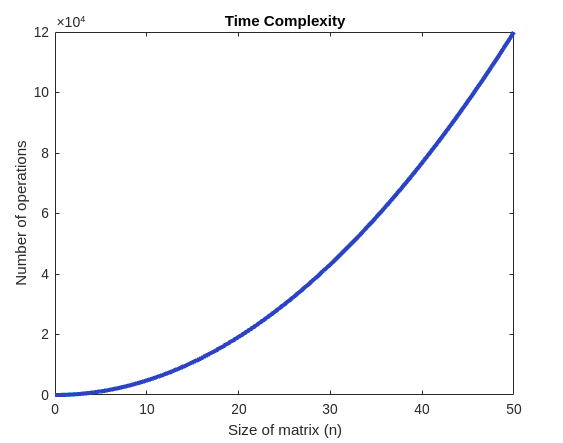
\includegraphics[width=3.12in,height=2.46in]{./image1.png}
	\end{Center}
\end{figure}


%%%%%%%%%%%%%%%%%%%% Figure/Image No: 1 Ends here %%%%%%%%%%%%%%%%%%%%


\vspace{\baselineskip}\begin{justify}
\textbf{Graph for Space Complexity}
\end{justify}

\vspace{\baselineskip}
\begin{Center}
\textbf{FIGURE 2}
\end{Center}


%%%%%%%%%%%%%%%%%%%% Figure/Image No: 2 starts here %%%%%%%%%%%%%%%%%%%%

\begin{figure}[H]
	\begin{Center}
		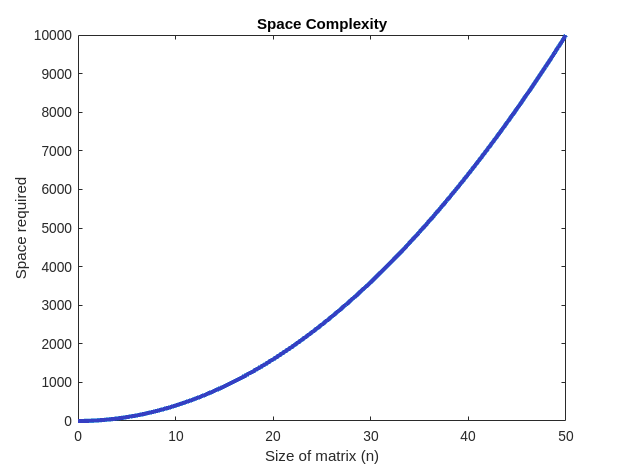
\includegraphics[width=3.12in,height=2.38in]{./image2.png}
	\end{Center}
\end{figure}


%%%%%%%%%%%%%%%%%%%% Figure/Image No: 2 Ends here %%%%%%%%%%%%%%%%%%%%


\vspace{\baselineskip}
\vspace{\baselineskip}

\vspace{\baselineskip}

\vspace{\baselineskip}
	\item {\fontsize{15pt}{18.0pt}\selectfont \textbf{CONCLUSION}}

\vspace{\baselineskip}
\begin{justify}
We have used a divide and conquer approach with the motive to reduce the time and space complexity of the algorithm. But we find that despite using divide and conquer approach our complexity is similar to a version using brute force for solving the same problem. Also in some cases the brute force version can give in fact a better time complexity with respect to divide and conquer approach.
\end{justify}
\begin{justify}
Their are also some cases in which the divide and conquer approach will give a whopping time complexity of Log(n) but in the average case time complexity of divide and conquer is a constant times greater than that of brute force.
\end{justify}
\begin{justify}
So we can conclude that divide and conquer approach in this problem is a failure as brute force approach is a better approach than divide and conquer.
\end{justify}

\vspace{\baselineskip}

\vspace{\baselineskip}

\vspace{\baselineskip}

\vspace{\baselineskip}
	\item {\fontsize{15pt}{18.0pt}\selectfont \textbf{REFERENCES}}
\end{enumerate}

\vspace{\baselineskip}
\begin{enumerate}
	\item Introduction to Algorithms (MIT Press) by T H Cormen, C E Leiserson, R L Rivest, and C Stein 
	\item \href{https://en.wikipedia.org/wiki/Divide-and-conquer_algorithm}{\textcolor[HTML]{1155CC}{\ul{https://en.wikipedia.org/wiki/Divide-and-conquer\_algorithm}}}
	\item \href{https://matlab.mathworks.com/}{\textcolor[HTML]{1155CC}{\ul{https://matlab.mathworks.com/}}}
\end{enumerate}

\vspace{\baselineskip}

\vspace{\baselineskip}

\vspace{\baselineskip}

\vspace{\baselineskip}

\end{multicols}
\printbibliography
\end{document}
